\documentclass[twoside]{book}

% Packages required by doxygen
\usepackage{calc}
\usepackage{doxygen}
\usepackage{graphicx}
\usepackage[utf8]{inputenc}
\usepackage{makeidx}
\usepackage{multicol}
\usepackage{multirow}
\usepackage{textcomp}
\usepackage[table]{xcolor}

% Font selection
\usepackage[T1]{fontenc}
\usepackage{mathptmx}
\usepackage[scaled=.90]{helvet}
\usepackage{courier}
\usepackage{amssymb}
\usepackage{sectsty}
\renewcommand{\familydefault}{\sfdefault}
\allsectionsfont{%
  \fontseries{bc}\selectfont%
  \color{darkgray}%
}
\renewcommand{\DoxyLabelFont}{%
  \fontseries{bc}\selectfont%
  \color{darkgray}%
}

% Page & text layout
\usepackage{geometry}
\geometry{%
  a4paper,%
  top=2.5cm,%
  bottom=2.5cm,%
  left=2.5cm,%
  right=2.5cm%
}
\tolerance=750
\hfuzz=15pt
\hbadness=750
\setlength{\emergencystretch}{15pt}
\setlength{\parindent}{0cm}
\setlength{\parskip}{0.2cm}
\makeatletter
\renewcommand{\paragraph}{%
  \@startsection{paragraph}{4}{0ex}{-1.0ex}{1.0ex}{%
    \normalfont\normalsize\bfseries\SS@parafont%
  }%
}
\renewcommand{\subparagraph}{%
  \@startsection{subparagraph}{5}{0ex}{-1.0ex}{1.0ex}{%
    \normalfont\normalsize\bfseries\SS@subparafont%
  }%
}
\makeatother

% Headers & footers
\usepackage{fancyhdr}
\pagestyle{fancyplain}
\fancyhead[LE]{\fancyplain{}{\bfseries\thepage}}
\fancyhead[CE]{\fancyplain{}{}}
\fancyhead[RE]{\fancyplain{}{\bfseries\leftmark}}
\fancyhead[LO]{\fancyplain{}{\bfseries\rightmark}}
\fancyhead[CO]{\fancyplain{}{}}
\fancyhead[RO]{\fancyplain{}{\bfseries\thepage}}
\fancyfoot[LE]{\fancyplain{}{}}
\fancyfoot[CE]{\fancyplain{}{}}
\fancyfoot[RE]{\fancyplain{}{\bfseries\scriptsize Generated on Fri Nov 7 2014 11\-:07\-:37 for t\-C\-A\-D by Doxygen }}
\fancyfoot[LO]{\fancyplain{}{\bfseries\scriptsize Generated on Fri Nov 7 2014 11\-:07\-:37 for t\-C\-A\-D by Doxygen }}
\fancyfoot[CO]{\fancyplain{}{}}
\fancyfoot[RO]{\fancyplain{}{}}
\renewcommand{\footrulewidth}{0.4pt}
\renewcommand{\chaptermark}[1]{%
  \markboth{#1}{}%
}
\renewcommand{\sectionmark}[1]{%
  \markright{\thesection\ #1}%
}

% Indices & bibliography
\usepackage{natbib}
\usepackage[titles]{tocloft}
\setcounter{tocdepth}{3}
\setcounter{secnumdepth}{5}
\makeindex

% Hyperlinks (required, but should be loaded last)
\usepackage{ifpdf}
\ifpdf
  \usepackage[pdftex,pagebackref=true]{hyperref}
\else
  \usepackage[ps2pdf,pagebackref=true]{hyperref}
\fi
\hypersetup{%
  colorlinks=true,%
  linkcolor=blue,%
  citecolor=blue,%
  unicode%
}

% Custom commands
\newcommand{\clearemptydoublepage}{%
  \newpage{\pagestyle{empty}\cleardoublepage}%
}


%===== C O N T E N T S =====

\begin{document}

% Titlepage & ToC
\hypersetup{pageanchor=false}
\pagenumbering{roman}
\begin{titlepage}
\vspace*{7cm}
\begin{center}%
{\Large t\-C\-A\-D \\[1ex]\large 0.\-2 }\\
\vspace*{1cm}
{\large Generated by Doxygen 1.8.6}\\
\vspace*{0.5cm}
{\small Fri Nov 7 2014 11:07:37}\\
\end{center}
\end{titlepage}
\clearemptydoublepage
\tableofcontents
\clearemptydoublepage
\pagenumbering{arabic}
\hypersetup{pageanchor=true}

%--- Begin generated contents ---
\chapter{Hierarchical Index}
\section{Class Hierarchy}
This inheritance list is sorted roughly, but not completely, alphabetically\-:\begin{DoxyCompactList}
\item \contentsline{section}{arc}{\pageref{classarc}}{}
\begin{DoxyCompactList}
\item \contentsline{section}{entities}{\pageref{classentities}}{}
\end{DoxyCompactList}
\item \contentsline{section}{circle}{\pageref{classcircle}}{}
\begin{DoxyCompactList}
\item \contentsline{section}{entities}{\pageref{classentities}}{}
\end{DoxyCompactList}
\item \contentsline{section}{line}{\pageref{classline}}{}
\begin{DoxyCompactList}
\item \contentsline{section}{entities}{\pageref{classentities}}{}
\end{DoxyCompactList}
\end{DoxyCompactList}

\chapter{Class Index}
\section{Class List}
Here are the classes, structs, unions and interfaces with brief descriptions\-:\begin{DoxyCompactList}
\item\contentsline{section}{\hyperlink{classarc}{arc} }{\pageref{classarc}}{}
\item\contentsline{section}{\hyperlink{classcircle}{circle} }{\pageref{classcircle}}{}
\item\contentsline{section}{\hyperlink{classentities}{entities} }{\pageref{classentities}}{}
\item\contentsline{section}{\hyperlink{classline}{line} }{\pageref{classline}}{}
\end{DoxyCompactList}

\chapter{File Index}
\section{File List}
Here is a list of all documented files with brief descriptions\-:\begin{DoxyCompactList}
\item\contentsline{section}{\hyperlink{arc_8h}{arc.\-h} \\*Adding arc entities }{\pageref{arc_8h}}{}
\item\contentsline{section}{\hyperlink{circle_8h}{circle.\-h} \\*Adding circle entities }{\pageref{circle_8h}}{}
\item\contentsline{section}{\hyperlink{draw_8h}{draw.\-h} \\*Implementation of drawing entities to backend }{\pageref{draw_8h}}{}
\item\contentsline{section}{\hyperlink{entities_8h}{entities.\-h} \\*Class which encapsulates all entities }{\pageref{entities_8h}}{}
\item\contentsline{section}{\hyperlink{line_8h}{line.\-h} \\*Adding line entities }{\pageref{line_8h}}{}
\item\contentsline{section}{\hyperlink{main_8cc}{main.\-cc} \\*Main Method }{\pageref{main_8cc}}{}
\end{DoxyCompactList}

\chapter{Class Documentation}
\hypertarget{classarc}{\section{arc Class Reference}
\label{classarc}\index{arc@{arc}}
}
Inheritance diagram for arc\-:\begin{figure}[H]
\begin{center}
\leavevmode
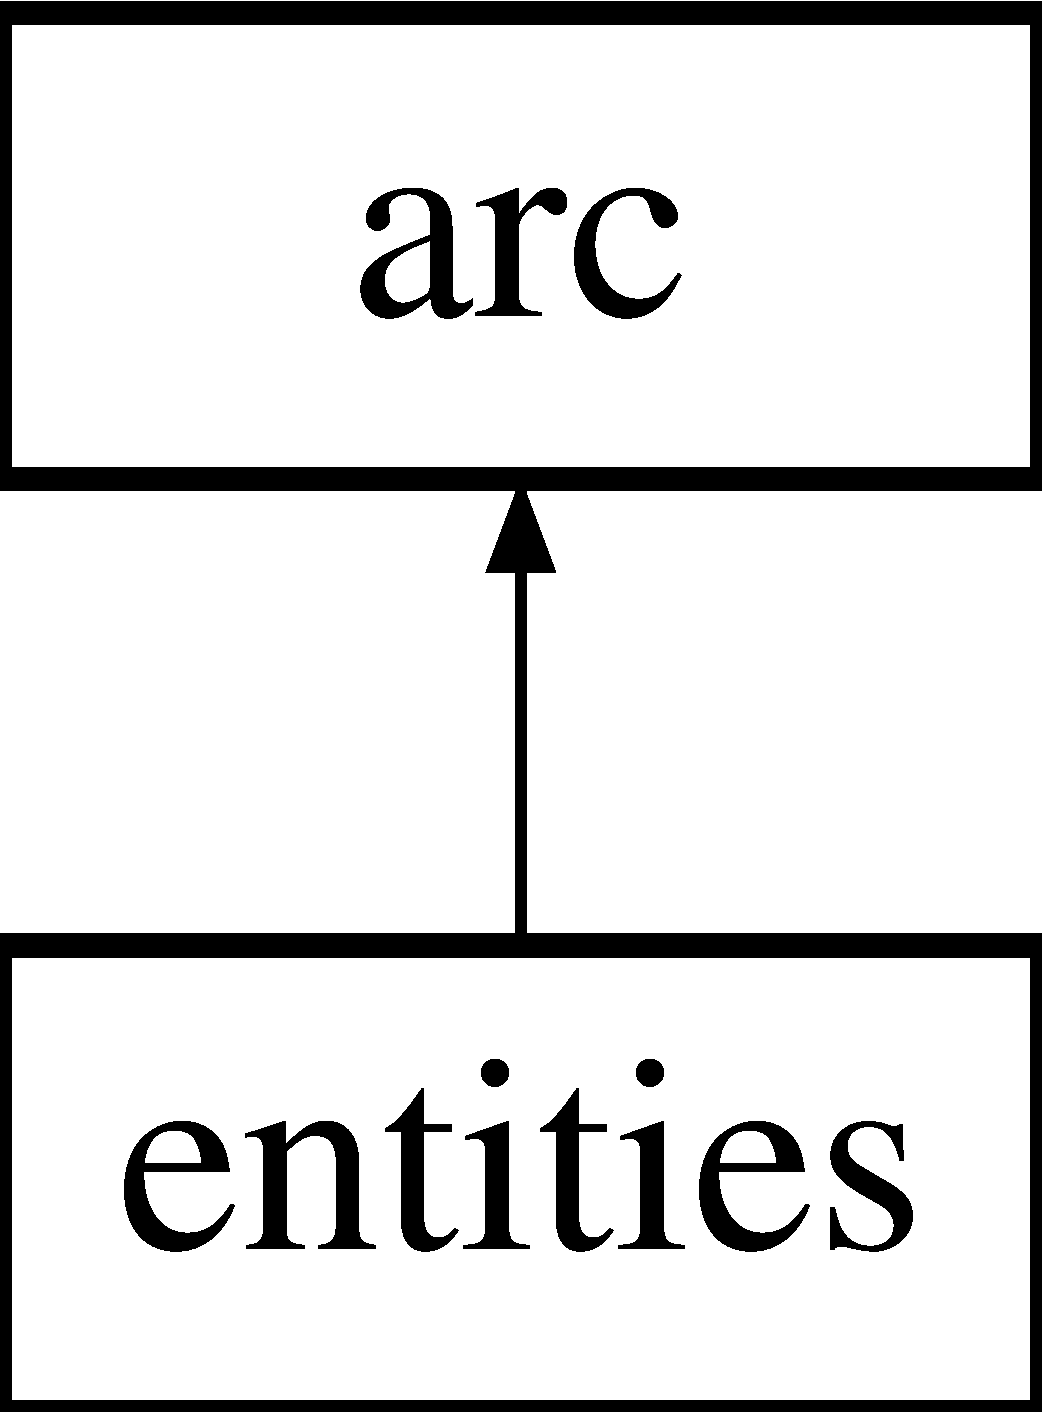
\includegraphics[height=2.000000cm]{classarc}
\end{center}
\end{figure}
\subsection*{Public Member Functions}
\begin{DoxyCompactItemize}
\item 
int \hyperlink{classarc_a42b9d162dd9b2b43b473c7d4a3de6b18}{no\-\_\-arc} (void)
\item 
void \hyperlink{classarc_a4adbfcd69160359a6aa314a56cf4cbaa}{get\-\_\-arc\-\_\-data} (void)
\item 
void \hyperlink{classarc_a0d8515bf57d53f2dffdb335c4377d841}{show\-\_\-arc} (void)
\item 
vector$<$ double $>$ \hyperlink{classarc_a73df92c812c6e50fed065aab910dc81d}{get\-\_\-arc\-\_\-vec} (void)
\end{DoxyCompactItemize}


\subsection{Member Function Documentation}
\hypertarget{classarc_a4adbfcd69160359a6aa314a56cf4cbaa}{\index{arc@{arc}!get\-\_\-arc\-\_\-data@{get\-\_\-arc\-\_\-data}}
\index{get\-\_\-arc\-\_\-data@{get\-\_\-arc\-\_\-data}!arc@{arc}}
\subsubsection[{get\-\_\-arc\-\_\-data}]{\setlength{\rightskip}{0pt plus 5cm}void arc\-::get\-\_\-arc\-\_\-data (
\begin{DoxyParamCaption}
\item[{void}]{}
\end{DoxyParamCaption}
)}}\label{classarc_a4adbfcd69160359a6aa314a56cf4cbaa}


 Class\-: arc Method\-: void arc \-:\-: \hyperlink{classarc_a4adbfcd69160359a6aa314a56cf4cbaa}{get\-\_\-arc\-\_\-data(void)} \subsubsection*{Description\-: Prompt for getting parameters of arc }\hypertarget{classarc_a73df92c812c6e50fed065aab910dc81d}{\index{arc@{arc}!get\-\_\-arc\-\_\-vec@{get\-\_\-arc\-\_\-vec}}
\index{get\-\_\-arc\-\_\-vec@{get\-\_\-arc\-\_\-vec}!arc@{arc}}
\subsubsection[{get\-\_\-arc\-\_\-vec}]{\setlength{\rightskip}{0pt plus 5cm}vector$<$ double $>$ arc\-::get\-\_\-arc\-\_\-vec (
\begin{DoxyParamCaption}
\item[{void}]{}
\end{DoxyParamCaption}
)}}\label{classarc_a73df92c812c6e50fed065aab910dc81d}


 Class\-: arc Method\-: vector$<$double$>$ arc \-:\-: \hyperlink{classarc_a73df92c812c6e50fed065aab910dc81d}{get\-\_\-arc\-\_\-vec(void)} \subsubsection*{Description\-: Returns a vector which contain all parameters }\hypertarget{classarc_a42b9d162dd9b2b43b473c7d4a3de6b18}{\index{arc@{arc}!no\-\_\-arc@{no\-\_\-arc}}
\index{no\-\_\-arc@{no\-\_\-arc}!arc@{arc}}
\subsubsection[{no\-\_\-arc}]{\setlength{\rightskip}{0pt plus 5cm}int arc\-::no\-\_\-arc (
\begin{DoxyParamCaption}
\item[{void}]{}
\end{DoxyParamCaption}
)}}\label{classarc_a42b9d162dd9b2b43b473c7d4a3de6b18}


 Class\-: arc Method\-: int arc \-:\-: \hyperlink{classarc_a42b9d162dd9b2b43b473c7d4a3de6b18}{no\-\_\-arc(void)} \subsubsection*{Description\-: Return number of arcs saved in memory }\hypertarget{classarc_a0d8515bf57d53f2dffdb335c4377d841}{\index{arc@{arc}!show\-\_\-arc@{show\-\_\-arc}}
\index{show\-\_\-arc@{show\-\_\-arc}!arc@{arc}}
\subsubsection[{show\-\_\-arc}]{\setlength{\rightskip}{0pt plus 5cm}void arc\-::show\-\_\-arc (
\begin{DoxyParamCaption}
\item[{void}]{}
\end{DoxyParamCaption}
)}}\label{classarc_a0d8515bf57d53f2dffdb335c4377d841}


 Class\-: arc Method\-: void arc \-:\-: \hyperlink{classarc_a0d8515bf57d53f2dffdb335c4377d841}{show\-\_\-arc(void)} \subsubsection*{Description\-: Show all arcs saved in memory }

The documentation for this class was generated from the following files\-:\begin{DoxyCompactItemize}
\item 
\hyperlink{arc_8h}{arc.\-h}\item 
arc.\-cc\end{DoxyCompactItemize}

\hypertarget{classcircle}{\section{circle Class Reference}
\label{classcircle}\index{circle@{circle}}
}
Inheritance diagram for circle\-:\begin{figure}[H]
\begin{center}
\leavevmode
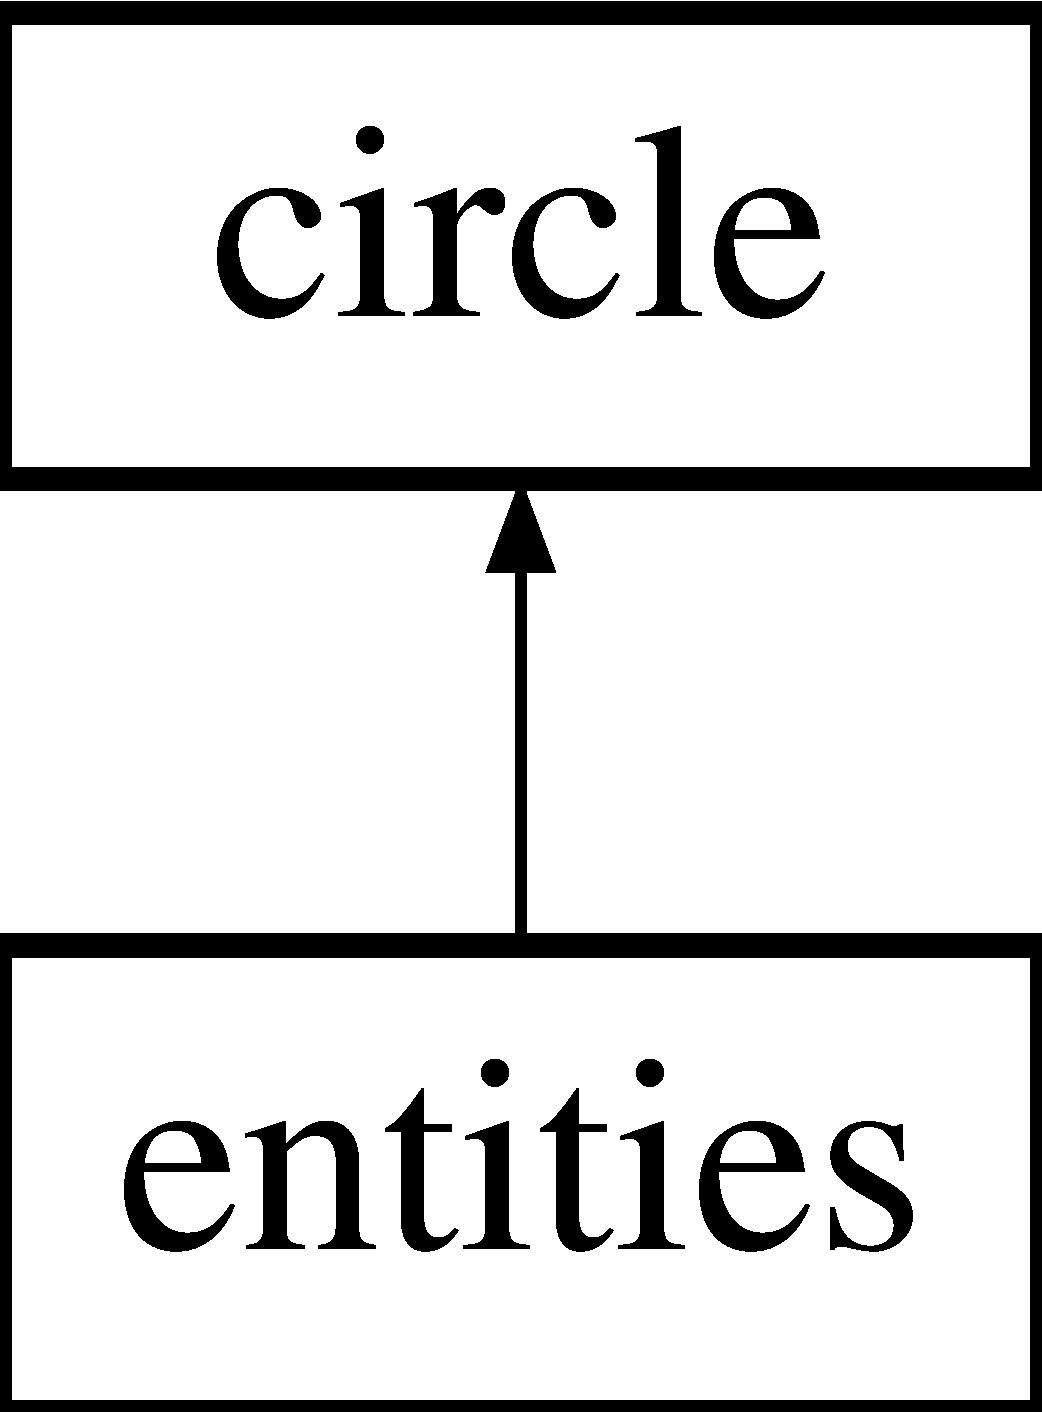
\includegraphics[height=2.000000cm]{classcircle}
\end{center}
\end{figure}
\subsection*{Public Member Functions}
\begin{DoxyCompactItemize}
\item 
int \hyperlink{classcircle_ac9e8a32e4f4a2cd2f5d9f61356a8a8e7}{no\-\_\-circle} ()
\item 
void \hyperlink{classcircle_ae2a965081be5a1bc8ba70078e8b4f269}{get\-\_\-circle\-\_\-data} ()
\item 
void \hyperlink{classcircle_afdb7bb3662cddd77e7385961ce365f2c}{show\-\_\-circle} ()
\item 
vector$<$ double $>$ \hyperlink{classcircle_a6253c4846df1bc44db16f8d2ae47b056}{get\-\_\-circle\-\_\-vec} ()
\end{DoxyCompactItemize}


\subsection{Member Function Documentation}
\hypertarget{classcircle_ae2a965081be5a1bc8ba70078e8b4f269}{\index{circle@{circle}!get\-\_\-circle\-\_\-data@{get\-\_\-circle\-\_\-data}}
\index{get\-\_\-circle\-\_\-data@{get\-\_\-circle\-\_\-data}!circle@{circle}}
\subsubsection[{get\-\_\-circle\-\_\-data}]{\setlength{\rightskip}{0pt plus 5cm}void circle\-::get\-\_\-circle\-\_\-data (
\begin{DoxyParamCaption}
{}
\end{DoxyParamCaption}
)}}\label{classcircle_ae2a965081be5a1bc8ba70078e8b4f269}


 Class\-: circle Method\-: void circle \-:\-: \hyperlink{classcircle_ae2a965081be5a1bc8ba70078e8b4f269}{get\-\_\-circle\-\_\-data(void)} \subsubsection*{Description\-: Prompt for getting parameters of circle }\hypertarget{classcircle_a6253c4846df1bc44db16f8d2ae47b056}{\index{circle@{circle}!get\-\_\-circle\-\_\-vec@{get\-\_\-circle\-\_\-vec}}
\index{get\-\_\-circle\-\_\-vec@{get\-\_\-circle\-\_\-vec}!circle@{circle}}
\subsubsection[{get\-\_\-circle\-\_\-vec}]{\setlength{\rightskip}{0pt plus 5cm}vector$<$ double $>$ circle\-::get\-\_\-circle\-\_\-vec (
\begin{DoxyParamCaption}
{}
\end{DoxyParamCaption}
)}}\label{classcircle_a6253c4846df1bc44db16f8d2ae47b056}


 Class\-: circle Method\-: vector$<$double$>$ circle \-:\-: \hyperlink{classcircle_a6253c4846df1bc44db16f8d2ae47b056}{get\-\_\-circle\-\_\-vec(void)} \subsubsection*{Description\-: Returns a vector which contain all parameters }\hypertarget{classcircle_ac9e8a32e4f4a2cd2f5d9f61356a8a8e7}{\index{circle@{circle}!no\-\_\-circle@{no\-\_\-circle}}
\index{no\-\_\-circle@{no\-\_\-circle}!circle@{circle}}
\subsubsection[{no\-\_\-circle}]{\setlength{\rightskip}{0pt plus 5cm}int circle\-::no\-\_\-circle (
\begin{DoxyParamCaption}
{}
\end{DoxyParamCaption}
)}}\label{classcircle_ac9e8a32e4f4a2cd2f5d9f61356a8a8e7}


 Class\-: circle Method\-: int circle \-:\-: \hyperlink{classcircle_ac9e8a32e4f4a2cd2f5d9f61356a8a8e7}{no\-\_\-circle(void)} \subsubsection*{Description\-: Return number of circles saved in memory }\hypertarget{classcircle_afdb7bb3662cddd77e7385961ce365f2c}{\index{circle@{circle}!show\-\_\-circle@{show\-\_\-circle}}
\index{show\-\_\-circle@{show\-\_\-circle}!circle@{circle}}
\subsubsection[{show\-\_\-circle}]{\setlength{\rightskip}{0pt plus 5cm}void circle\-::show\-\_\-circle (
\begin{DoxyParamCaption}
{}
\end{DoxyParamCaption}
)}}\label{classcircle_afdb7bb3662cddd77e7385961ce365f2c}


 Class\-: circle Method\-: void circle \-:\-: \hyperlink{classcircle_afdb7bb3662cddd77e7385961ce365f2c}{show\-\_\-circle(void)} \subsubsection*{Description\-: Show all circles saved in memory }

The documentation for this class was generated from the following files\-:\begin{DoxyCompactItemize}
\item 
\hyperlink{circle_8h}{circle.\-h}\item 
circle.\-cc\end{DoxyCompactItemize}

\hypertarget{classentities}{\section{entities Class Reference}
\label{classentities}\index{entities@{entities}}
}
Inheritance diagram for entities\-:\begin{figure}[H]
\begin{center}
\leavevmode
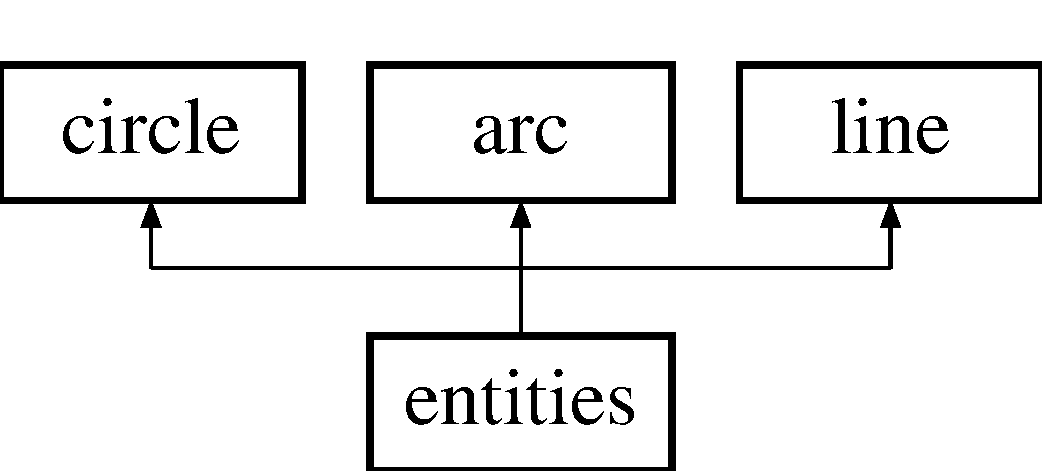
\includegraphics[height=2.000000cm]{classentities}
\end{center}
\end{figure}
\subsection*{Public Member Functions}
\begin{DoxyCompactItemize}
\item 
\hypertarget{classentities_ae7df80d4007a075181244f8c2f2dd6f6}{void {\bfseries show} ()}\label{classentities_ae7df80d4007a075181244f8c2f2dd6f6}

\end{DoxyCompactItemize}


The documentation for this class was generated from the following file\-:\begin{DoxyCompactItemize}
\item 
\hyperlink{entities_8h}{entities.\-h}\end{DoxyCompactItemize}

\hypertarget{classline}{\section{line Class Reference}
\label{classline}\index{line@{line}}
}
Inheritance diagram for line\-:\begin{figure}[H]
\begin{center}
\leavevmode
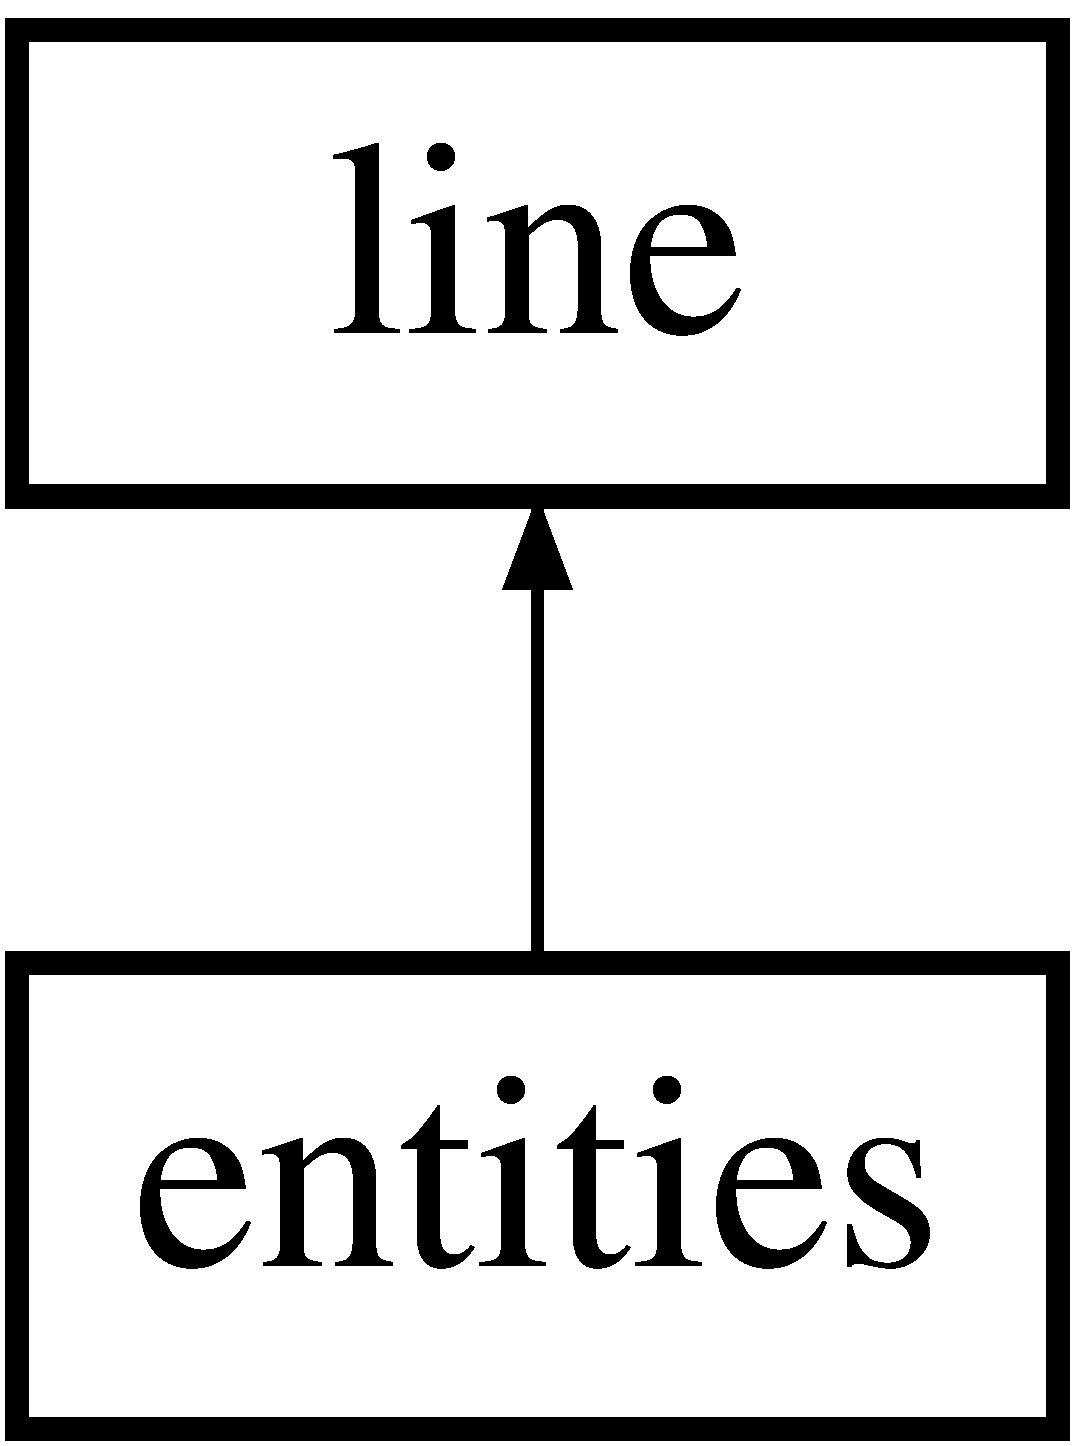
\includegraphics[height=2.000000cm]{classline}
\end{center}
\end{figure}
\subsection*{Public Member Functions}
\begin{DoxyCompactItemize}
\item 
int \hyperlink{classline_a3bf13756439854a27a7c967a3dfaec00}{no\-\_\-line} ()
\item 
void \hyperlink{classline_a33a0c7a89f4621d61d334924371fb647}{get\-\_\-line\-\_\-data} ()
\item 
void \hyperlink{classline_aee425c3dfb103b45b468693e85fbaa30}{show\-\_\-line} ()
\item 
vector$<$ double $>$ \hyperlink{classline_ab52b48d96bec47e593045a14262581b4}{get\-\_\-line\-\_\-vec} ()
\end{DoxyCompactItemize}


\subsection{Member Function Documentation}
\hypertarget{classline_a33a0c7a89f4621d61d334924371fb647}{\index{line@{line}!get\-\_\-line\-\_\-data@{get\-\_\-line\-\_\-data}}
\index{get\-\_\-line\-\_\-data@{get\-\_\-line\-\_\-data}!line@{line}}
\subsubsection[{get\-\_\-line\-\_\-data}]{\setlength{\rightskip}{0pt plus 5cm}void line\-::get\-\_\-line\-\_\-data (
\begin{DoxyParamCaption}
{}
\end{DoxyParamCaption}
)}}\label{classline_a33a0c7a89f4621d61d334924371fb647}


 Class\-: line Method\-: void line \-:\-: \hyperlink{classline_a33a0c7a89f4621d61d334924371fb647}{get\-\_\-line\-\_\-data(void)} \subsubsection*{Description\-: Prompt for getting parameters of line }\hypertarget{classline_ab52b48d96bec47e593045a14262581b4}{\index{line@{line}!get\-\_\-line\-\_\-vec@{get\-\_\-line\-\_\-vec}}
\index{get\-\_\-line\-\_\-vec@{get\-\_\-line\-\_\-vec}!line@{line}}
\subsubsection[{get\-\_\-line\-\_\-vec}]{\setlength{\rightskip}{0pt plus 5cm}vector$<$ double $>$ line\-::get\-\_\-line\-\_\-vec (
\begin{DoxyParamCaption}
{}
\end{DoxyParamCaption}
)}}\label{classline_ab52b48d96bec47e593045a14262581b4}


 Class\-: line Method\-: vector$<$double$>$ line \-:\-: \hyperlink{classline_ab52b48d96bec47e593045a14262581b4}{get\-\_\-line\-\_\-vec(void)} \subsubsection*{Description\-: Returns a vector which contain all parameters }\hypertarget{classline_a3bf13756439854a27a7c967a3dfaec00}{\index{line@{line}!no\-\_\-line@{no\-\_\-line}}
\index{no\-\_\-line@{no\-\_\-line}!line@{line}}
\subsubsection[{no\-\_\-line}]{\setlength{\rightskip}{0pt plus 5cm}int line\-::no\-\_\-line (
\begin{DoxyParamCaption}
{}
\end{DoxyParamCaption}
)}}\label{classline_a3bf13756439854a27a7c967a3dfaec00}


 Class\-: line Method\-: int line \-:\-: \hyperlink{classline_a3bf13756439854a27a7c967a3dfaec00}{no\-\_\-line(void)} \subsubsection*{Description\-: Return number of lines saved in memory }\hypertarget{classline_aee425c3dfb103b45b468693e85fbaa30}{\index{line@{line}!show\-\_\-line@{show\-\_\-line}}
\index{show\-\_\-line@{show\-\_\-line}!line@{line}}
\subsubsection[{show\-\_\-line}]{\setlength{\rightskip}{0pt plus 5cm}void line\-::show\-\_\-line (
\begin{DoxyParamCaption}
{}
\end{DoxyParamCaption}
)}}\label{classline_aee425c3dfb103b45b468693e85fbaa30}


 Class\-: line Method\-: void line \-:\-: \hyperlink{classline_aee425c3dfb103b45b468693e85fbaa30}{show\-\_\-line(void)} \subsubsection*{Description\-: Show all lines saved in memory }

The documentation for this class was generated from the following files\-:\begin{DoxyCompactItemize}
\item 
\hyperlink{line_8h}{line.\-h}\item 
line.\-cc\end{DoxyCompactItemize}

\chapter{File Documentation}
\hypertarget{arc_8h}{\section{arc.\-h File Reference}
\label{arc_8h}\index{arc.\-h@{arc.\-h}}
}


Adding arc entities.  


{\ttfamily \#include $<$iostream$>$}\\*
{\ttfamily \#include $<$vector$>$}\\*
{\ttfamily \#include $<$cmath$>$}\\*
\subsection*{Classes}
\begin{DoxyCompactItemize}
\item 
class \hyperlink{classarc}{arc}
\end{DoxyCompactItemize}


\subsection{Detailed Description}
Adding arc entities. \begin{DoxyVersion}{Version}
0.\-2 \textbackslash{} 
\end{DoxyVersion}
\begin{DoxyAuthor}{Author}
Jagmeet Singh, \href{mailto:jagmeet787@gmail.com}{\tt jagmeet787@gmail.\-com} 
\end{DoxyAuthor}
\begin{DoxyCopyright}{Copyright}
Copyright (c) 2013, Jagmeet Singh \href{https://github.com/jagmeet787}{\tt https\-://github.\-com/jagmeet787} 
\end{DoxyCopyright}

\hypertarget{circle_8h}{\section{circle.\-h File Reference}
\label{circle_8h}\index{circle.\-h@{circle.\-h}}
}


Adding circle entities.  


{\ttfamily \#include $<$iostream$>$}\\*
{\ttfamily \#include $<$vector$>$}\\*
{\ttfamily \#include $<$cmath$>$}\\*
\subsection*{Classes}
\begin{DoxyCompactItemize}
\item 
class \hyperlink{classcircle}{circle}
\end{DoxyCompactItemize}


\subsection{Detailed Description}
Adding circle entities. \begin{DoxyVersion}{Version}
0.\-2 \textbackslash{} 
\end{DoxyVersion}
\begin{DoxyAuthor}{Author}
Jagmeet Singh, \href{mailto:jagmeet787@gmail.com}{\tt jagmeet787@gmail.\-com} 
\end{DoxyAuthor}
\begin{DoxyCopyright}{Copyright}
Copyright (c) 2013, Jagmeet Singh \href{https://github.com/jagmeet787}{\tt https\-://github.\-com/jagmeet787} 
\end{DoxyCopyright}

\hypertarget{draw_8h}{\section{draw.\-h File Reference}
\label{draw_8h}\index{draw.\-h@{draw.\-h}}
}


Implementation of drawing entities to backend.  


{\ttfamily \#include $<$iostream$>$}\\*
{\ttfamily \#include $<$vector$>$}\\*
{\ttfamily \#include $<$cairo/cairo-\/pdf.\-h$>$}\\*
{\ttfamily \#include \char`\"{}lc/lccairopainter.\-h\char`\"{}}\\*
{\ttfamily \#include \char`\"{}entities.\-h\char`\"{}}\\*
\subsection*{Functions}
\begin{DoxyCompactItemize}
\item 
\hypertarget{draw_8h_a1664d54d81c6fed9ccc53bd2bf031992}{Lc\-Cairo\-Painter {\bfseries lcpainter} (surface, cr)}\label{draw_8h_a1664d54d81c6fed9ccc53bd2bf031992}

\item 
\hypertarget{draw_8h_a30dbc0614efcd06921afc7dc9104b3e4}{void {\bfseries drawline} (void)}\label{draw_8h_a30dbc0614efcd06921afc7dc9104b3e4}

\item 
\hypertarget{draw_8h_a2fd98ea12c282136f08e1d09d1acd756}{void {\bfseries drawarc} (void)}\label{draw_8h_a2fd98ea12c282136f08e1d09d1acd756}

\item 
\hypertarget{draw_8h_ac70f9b47b10989ee37a26ecfee600252}{void {\bfseries drawcircle} (void)}\label{draw_8h_ac70f9b47b10989ee37a26ecfee600252}

\item 
\hypertarget{draw_8h_a56c5cf8a568cff737ff95520cbe6b405}{void {\bfseries draw} ()}\label{draw_8h_a56c5cf8a568cff737ff95520cbe6b405}

\end{DoxyCompactItemize}
\subsection*{Variables}
\begin{DoxyCompactItemize}
\item 
\hypertarget{draw_8h_ab3b66c3ade85e8106f4634a4693e36d5}{\hyperlink{classentities}{entities} {\bfseries obj}}\label{draw_8h_ab3b66c3ade85e8106f4634a4693e36d5}

\item 
\hypertarget{draw_8h_a4ccc2ef4a43c6291071f905093b5d19b}{vector$<$ double $>$ {\bfseries line\-\_\-data} = obj.\-get\-\_\-line\-\_\-vec()}\label{draw_8h_a4ccc2ef4a43c6291071f905093b5d19b}

\item 
\hypertarget{draw_8h_a0d1bf92234761f10d76199a964c81558}{vector$<$ double $>$ {\bfseries arc\-\_\-data} = obj.\-get\-\_\-arc\-\_\-vec()}\label{draw_8h_a0d1bf92234761f10d76199a964c81558}

\item 
\hypertarget{draw_8h_ab36ed22f914afc411d24ff03f2dd843d}{vector$<$ double $>$ {\bfseries circle\-\_\-data} = obj.\-get\-\_\-circle\-\_\-vec()}\label{draw_8h_ab36ed22f914afc411d24ff03f2dd843d}

\item 
\hypertarget{draw_8h_a76e6dbb8b33b4373ca91aab3cab86245}{cairo\-\_\-surface\-\_\-t $\ast$ {\bfseries surface} =(cairo\-\_\-surface\-\_\-t $\ast$)cairo\-\_\-pdf\-\_\-surface\-\_\-create(\char`\"{}ji.\-pdf\char`\"{},100,100)}\label{draw_8h_a76e6dbb8b33b4373ca91aab3cab86245}

\item 
\hypertarget{draw_8h_ac2efa4a51d11834112524e53b3dc0f62}{cairo\-\_\-t $\ast$ {\bfseries cr} = cairo\-\_\-create(surface)}\label{draw_8h_ac2efa4a51d11834112524e53b3dc0f62}

\end{DoxyCompactItemize}


\subsection{Detailed Description}
Implementation of drawing entities to backend. \begin{DoxyVersion}{Version}
0.\-2 \textbackslash{} 
\end{DoxyVersion}
\begin{DoxyAuthor}{Author}
Jagmeet Singh, \href{mailto:jagmeet787@gmail.com}{\tt jagmeet787@gmail.\-com} 
\end{DoxyAuthor}
\begin{DoxyCopyright}{Copyright}
Copyright (c) 2013, Jagmeet Singh \href{https://github.com/jagmeet787}{\tt https\-://github.\-com/jagmeet787} 
\end{DoxyCopyright}

\hypertarget{entities_8h}{\section{entities.\-h File Reference}
\label{entities_8h}\index{entities.\-h@{entities.\-h}}
}


Class which encapsulates all entities.  


{\ttfamily \#include $<$iostream$>$}\\*
{\ttfamily \#include $<$vector$>$}\\*
{\ttfamily \#include $<$cstdlib$>$}\\*
{\ttfamily \#include \char`\"{}line.\-h\char`\"{}}\\*
{\ttfamily \#include \char`\"{}arc.\-h\char`\"{}}\\*
{\ttfamily \#include \char`\"{}circle.\-h\char`\"{}}\\*
\subsection*{Classes}
\begin{DoxyCompactItemize}
\item 
class \hyperlink{classentities}{entities}
\end{DoxyCompactItemize}


\subsection{Detailed Description}
Class which encapsulates all entities. \begin{DoxyVersion}{Version}
0.\-2 \textbackslash{} 
\end{DoxyVersion}
\begin{DoxyAuthor}{Author}
Jagmeet Singh, \href{mailto:jagmeet787@gmail.com}{\tt jagmeet787@gmail.\-com} 
\end{DoxyAuthor}
\begin{DoxyCopyright}{Copyright}
Copyright (c) 2013, Jagmeet Singh \href{https://github.com/jagmeet787}{\tt https\-://github.\-com/jagmeet787} 
\end{DoxyCopyright}

\hypertarget{line_8h}{\section{line.\-h File Reference}
\label{line_8h}\index{line.\-h@{line.\-h}}
}


Adding line entities.  


{\ttfamily \#include $<$iostream$>$}\\*
{\ttfamily \#include $<$vector$>$}\\*
{\ttfamily \#include $<$cmath$>$}\\*
\subsection*{Classes}
\begin{DoxyCompactItemize}
\item 
class \hyperlink{classline}{line}
\end{DoxyCompactItemize}


\subsection{Detailed Description}
Adding line entities. \begin{DoxyVersion}{Version}
0.\-2 \textbackslash{} 
\end{DoxyVersion}
\begin{DoxyAuthor}{Author}
Jagmeet Singh, \href{mailto:jagmeet787@gmail.com}{\tt jagmeet787@gmail.\-com} 
\end{DoxyAuthor}
\begin{DoxyCopyright}{Copyright}
Copyright (c) 2013, Jagmeet Singh \href{https://github.com/jagmeet787}{\tt https\-://github.\-com/jagmeet787} 
\end{DoxyCopyright}

\hypertarget{main_8cc}{\section{main.\-cc File Reference}
\label{main_8cc}\index{main.\-cc@{main.\-cc}}
}


Main Method.  


{\ttfamily \#include $<$iostream$>$}\\*
{\ttfamily \#include $<$cstdlib$>$}\\*
{\ttfamily \#include \char`\"{}draw.\-h\char`\"{}}\\*
\subsection*{Functions}
\begin{DoxyCompactItemize}
\item 
\hypertarget{main_8cc_ae66f6b31b5ad750f1fe042a706a4e3d4}{int {\bfseries main} ()}\label{main_8cc_ae66f6b31b5ad750f1fe042a706a4e3d4}

\end{DoxyCompactItemize}


\subsection{Detailed Description}
Main Method. \begin{DoxyVersion}{Version}
0.\-2
\end{DoxyVersion}
\begin{DoxyAuthor}{Author}
Jagmeet Singh, \href{mailto:jagmeet787@gmail.com}{\tt jagmeet787@gmail.\-com} 
\end{DoxyAuthor}
\begin{DoxyCopyright}{Copyright}
Copyright (c) 2013, Jagmeet Singh \href{https://github.com/jagmeet787}{\tt https\-://github.\-com/jagmeet787} 
\end{DoxyCopyright}

%--- End generated contents ---

% Index
\newpage
\phantomsection
\addcontentsline{toc}{chapter}{Index}
\printindex

\end{document}
